\section{Stochastic Gradient Descent}
\frame{\tableofcontents[currentsection, hideothersubsections]}

\begin{frame}
\frametitle{SGD}

\begin{figure}
    \centering
    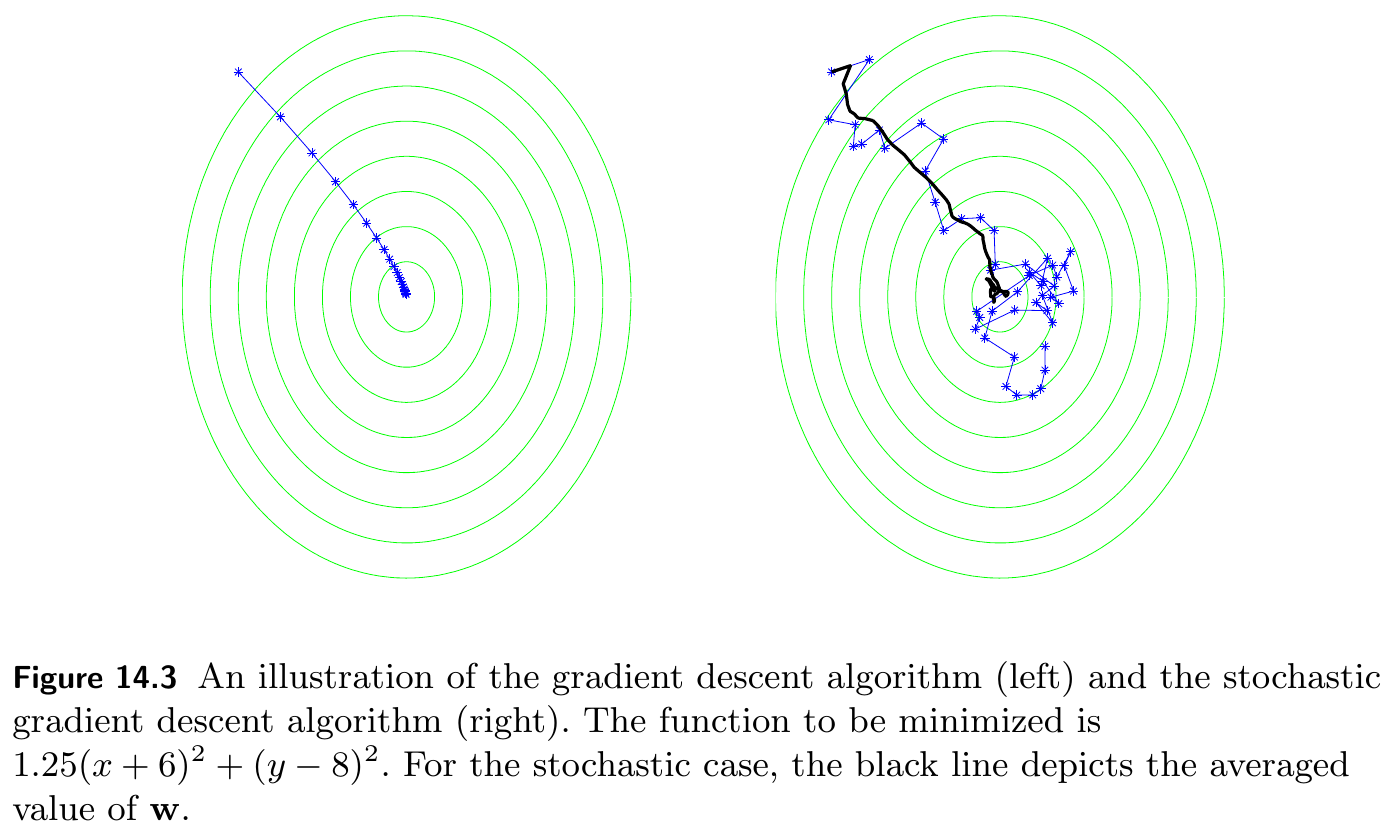
\includegraphics[scale=0.20]{fig_14_3}
\end{figure}

Stochastic GD:\\
the update direction to be a random vector and
only require that its expected value at each iteration will equal the gradient direction
(more generally, a subgradient of the function at the current vector)

\end{frame}

\begin{frame}
\frametitle{SGD}

\begin{figure}
    \centering
    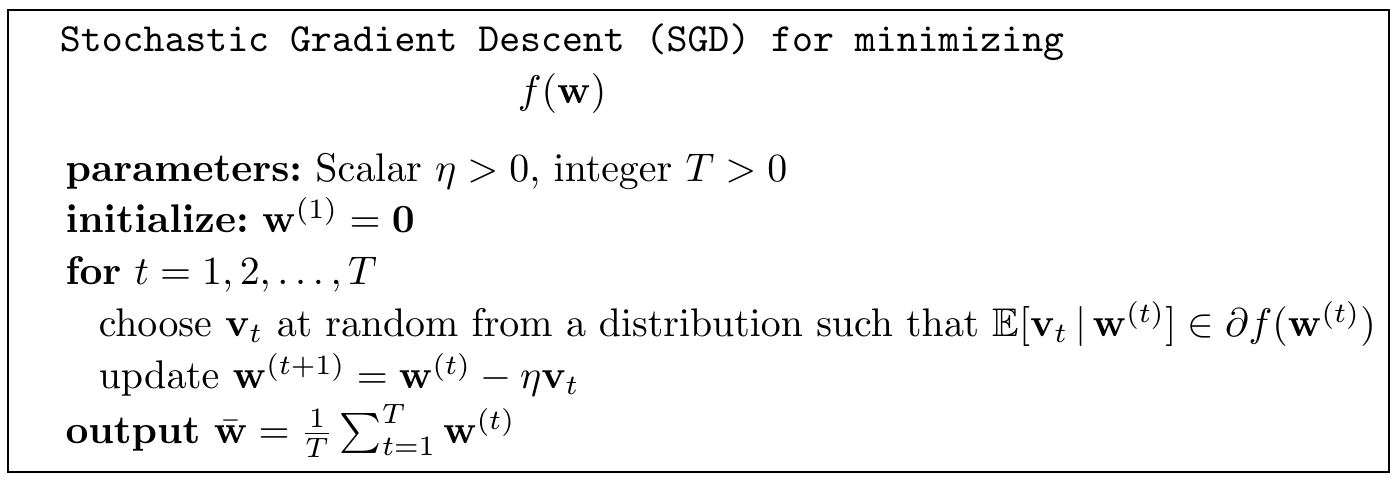
\includegraphics[scale=0.20]{sgd}
\end{figure}

\end{frame}
